\documentclass[11pt,compress,t,notes=noshow, xcolor=table]{beamer}
\usepackage[]{graphicx}\usepackage[]{color}
% maxwidth is the original width if it is less than linewidth
% otherwise use linewidth (to make sure the graphics do not exceed the margin)
\makeatletter
\def\maxwidth{ %
  \ifdim\Gin@nat@width>\linewidth
    \linewidth
  \else
    \Gin@nat@width
  \fi 
}
\makeatother

\definecolor{fgcolor}{rgb}{0.345, 0.345, 0.345}
\newcommand{\hlnum}[1]{\textcolor[rgb]{0.686,0.059,0.569}{#1}}%
\newcommand{\hlstr}[1]{\textcolor[rgb]{0.192,0.494,0.8}{#1}}%
\newcommand{\hlcom}[1]{\textcolor[rgb]{0.678,0.584,0.686}{\textit{#1}}}%
\newcommand{\hlopt}[1]{\textcolor[rgb]{0,0,0}{#1}}%
\newcommand{\hlstd}[1]{\textcolor[rgb]{0.345,0.345,0.345}{#1}}%
\newcommand{\hlkwa}[1]{\textcolor[rgb]{0.161,0.373,0.58}{\textbf{#1}}}%
\newcommand{\hlkwb}[1]{\textcolor[rgb]{0.69,0.353,0.396}{#1}}%
\newcommand{\hlkwc}[1]{\textcolor[rgb]{0.333,0.667,0.333}{#1}}%
\newcommand{\hlkwd}[1]{\textcolor[rgb]{0.737,0.353,0.396}{\textbf{#1}}}%
\let\hlipl\hlkwb

\usepackage{framed}
\makeatletter
\newenvironment{kframe}{%
 \def\at@end@of@kframe{}%
 \ifinner\ifhmode%
  \def\at@end@of@kframe{\end{minipage}}%
  \begin{minipage}{\columnwidth}%
 \fi\fi%
 \def\FrameCommand##1{\hskip\@totalleftmargin \hskip-\fboxsep
 \colorbox{shadecolor}{##1}\hskip-\fboxsep
     % There is no \\@totalrightmargin, so:
     \hskip-\linewidth \hskip-\@totalleftmargin \hskip\columnwidth}%
 \MakeFramed {\advance\hsize-\width
   \@totalleftmargin\z@ \linewidth\hsize
   \@setminipage}}%
 {\par\unskip\endMakeFramed%
 \at@end@of@kframe}
\makeatother

\definecolor{shadecolor}{rgb}{.97, .97, .97}
\definecolor{messagecolor}{rgb}{0, 0, 0}
\definecolor{warningcolor}{rgb}{1, 0, 1}
\definecolor{errorcolor}{rgb}{1, 0, 0}
\newenvironment{knitrout}{}{} % an empty environment to be redefined in TeX

\usepackage{alltt}
\newcommand{\SweaveOpts}[1]{}  % do not interfere with LaTeX
\newcommand{\SweaveInput}[1]{} % because they are not real TeX commands
\newcommand{\Sexpr}[1]{}       % will only be parsed by R



\usepackage[english]{babel}
\usepackage[utf8]{inputenc}

\usepackage{dsfont}
\usepackage{verbatim}
\usepackage{amsmath}
\usepackage{amsfonts}
\usepackage{bm}
\usepackage{csquotes}
\usepackage{multirow}
\usepackage{longtable}
\usepackage{booktabs}
\usepackage{enumerate}
\usepackage[absolute,overlay]{textpos}
\usepackage{psfrag}
\usepackage{algorithm}
\usepackage{algpseudocode}
\usepackage{eqnarray}
\usepackage{arydshln}
\usepackage{tabularx}
\usepackage{placeins}
\usepackage{tikz}
\usepackage{setspace}
\usepackage{colortbl}
\usepackage{mathtools}
\usepackage{wrapfig}
\usepackage{bm}
\usepackage{xcolor}
\usetikzlibrary{shapes,arrows,automata,positioning,calc,chains,trees, shadows}
\tikzset{
  %Define standard arrow tip
  >=stealth',
  %Define style for boxes
  punkt/.style={
    rectangle,
    rounded corners,
    draw=black, very thick,
    text width=6.5em,
    minimum height=2em,
    text centered},
  % Define arrow style
  pil/.style={
    ->,
    thick,
    shorten <=2pt,
    shorten >=2pt,}
}
\usepackage{subfig}


% Defines macros and environments
\input{../../style/common.tex}

%\usetheme{lmu-lecture}
% \newcommand{\titlefigure}{figure/ml-basic-riskmin-error-surface.png}
% \newcommand{\learninggoals}{\item Know the concept of loss \item Understand the relationship between loss and risk \item Understand the relationship between risk minimization and finding the best model}
\usepackage{fancy}

\colorlet{GRAY}{gray}

\let\code=\texttt
\let\proglang=\textsf

\setkeys{Gin}{width=0.9\textwidth}

\title{Introduction to Machine Learning}
% \author{Bernd Bischl, Christoph Molnar, Daniel Schalk, Fabian Scheipl}
\institute{\href{https://compstat-lmu.github.io/lecture_i2ml/}{compstat-lmu.github.io/lecture\_i2ml}}
\date{}

\setbeamertemplate{frametitle}{\expandafter\uppercase\expandafter\insertframetitle}



\begin{document}
% Introduction to Machine Learning
% Day 1

% Set style/preamble.Rnw as parent.

% Load all R packages and set up knitr

% This file loads R packages, configures knitr options and sets preamble.Rnw as parent file
% IF YOU MODIFY THIS, PLZ ALSO MODIFY setup.Rmd ACCORDINGLY...








% Defines macros and environments
\input{../../latex-math/basic-math.tex}
\input{../../latex-math/basic-ml.tex}
\input{../../latex-math/ml-lm.tex}

%! includes: basics-learners

\lecturechapter{ML-Basics: Losses \& Risk Minimization}
\lecture{Introduction to Machine Learning}

\begin{vbframe}{How to Evaluate Models}


 \end{vbframe}

\begin{frame}{Overview}

No Free Lunch
In machine learning, there’s something called the “No Free Lunch” theorem. In a nutshell, it states that no one algorithm works best for every problem, and it’s especially relevant for supervised learning (i.e. predictive modeling).

For example, you can’t say that neural networks are always better than decision trees or vice-versa. There are many factors at play, such as the size and structure of your dataset.

As a result, you should try many different algorithms for your problem, while using a hold-out “test set” of data to evaluate performance and select the winner.
\lz
\lz
Hypothesisspace + Risk + Optimization 
\end{frame}


% --------------------------------------------------------
% Linear model
% --------------------------------------------------------

\begin{vbframe}{Linear model ~~ Functionality}

\textbf{General information}
\begin{itemize}
\item one of the most common algorithms
\end{itemize}

\textbf{Aim}
\begin{itemize}
\item [Aim] Find the best line/straight hyperplane through data (LINEAR!)
\item Predict continuos, numeric variables
\end{itemize}

 
\textbf{Hypothesisspace}
$$\Hspace = \{ \theta_0 + \thx\ |\ (\theta_0, \thetab) \in \R^{p+1} \}$$

\centering 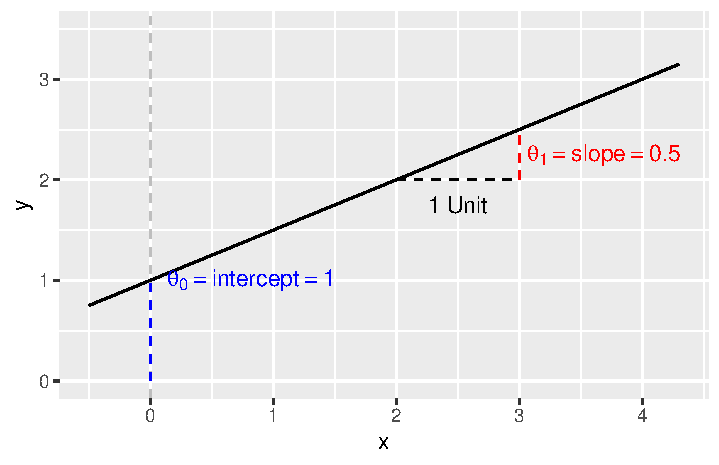
\includegraphics[width=0.4\textwidth]{figure/reg_lm_plot} 

\framebreak

\textbf{Risk}
\begin{itemize}
\item Empirical Risk Minimization with the loss function - normally quadratic loss fucntion 
\end{itemize}

\textbf{Optimization}

for L2-loss analytically; numerical optimization for others 


\lz

\textbf{Typical appication}




\end{vbframe}

\begin{frame}{Linear model - Advantages and Disadvantages}

\textbf{Advantages}
\begin{itemize}
\item simple implementation and simple to understand
\item interpretability: gives information about mean influence of the features --> feature importance
\item works good independent of dataset size
\item fits linearly separable datasets very good
\item cheap computational cost --> fast train and forecaste
\item ground for many other ML algorithms
\item fast training
\end{itemize}


\textbf{Disadvantages}
\begin{itemize}
\item strong assumptions: data is independent and normal-distributed(multicollinearity must be removed); simplification of real-world problems
\item overfitting --> can be reduced by regularization
\item sensitve to outliers and noisy data 
\item not suitable for non-linear data
\end{itemize}

\textbf{Conclusion}
Impressive results on lineare separable datasets with easy interpretation, but strong assumptions which do not apply on most of the real-world problems; oversimplifies it

\end{frame}
% ------------------------------------------------------------------------------



 %Logistic regression is the classification counterpart to linear regression. Predictions are mapped to be between 0 and 1 through the logistic function, which means that predictions can be interpreted as class probabilities.



% ------------------------------------------------------------------------------
% CART (Classification and Regression Trees)
% ------------------------------------------------------------------------------

\scriptsize

\begin{frame}{\textcolor{gray!80}{CART} ~~ Functionality}
\noindent \textcolor{gray!80}{\rule{\textwidth}{1pt}}

\vspace{0.3cm}

\textbf{\textcolor{gray!80}{General idea}} {} Starting from a root node, 
\textit{\textbf{classification \& regression trees (CART)}} 
perform repeated \textbf{binary splits} of the data according to feature values, 
thereby subsequently dividing the input space $\Xspace$ into $M$ 
\textbf{rectangular partitions}.

\begin{itemize}
  \item [$\rightarrow$] Pass observations along until each ends up in exactly 
  one leaf node
  \item [$\rightarrow$] In each step, find the optimal feature-threshold
  combination to split by
  \item [$\rightarrow$] Assign response $c_m$ to leaf node $m$
\end{itemize}

\vspace{0.3cm}

\begin{minipage}{0.6\textwidth}
  \textbf{\textcolor{gray!80}{Hypothesis space}} \\
  $$\Hspace = \left\{ \fx: \fx = \sum_{m = 1}^M c_m \mathbb{I}(\xv \in Q_m) 
  \right\}$$
  \smallskip
  \textbf{\textcolor{gray!80}{Loss functions}} \\
  Classification: \textit{\textbf{Brier score, Bernoulli loss}}  \\
  \smallskip
  Regression: \textit{\textbf{quadratic loss}} \\
  \smallskip
  \textbf{\textcolor{gray!80}{Optimization}} \\
  Exhaustive search for optimal splitting criterion
\end{minipage}%
\begin{minipage}{0.4\textwidth}
  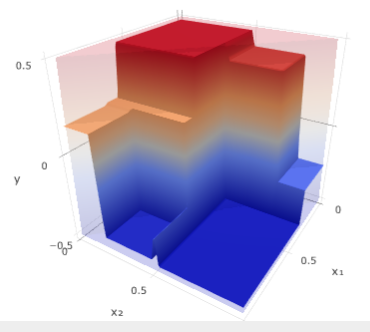
\includegraphics[width=\textwidth]{figure/cart_3d.PNG}
\end{minipage}

\vfill

\colorbox{gray!80}{\textcolor{white}{NON-PARAMETRIC}} 
\colorbox{gray!80}{\textcolor{white}{WHITE-BOX}} 
\colorbox{gray!80}{\textcolor{white}{FEATURE SELECTION}}

\end{frame}

% % ------------------------------------------------------------------------------

\begin{frame}{\textcolor{gray!60}{CART} ~~ APPLICATION}
\end{frame}

% ------------------------------------------------------------------------------


% --------------------------------------------------------
% RF   Random Forest 
% --------------------------------------------------------

\begin{frame}{Random Forest - Functionality}

\begin{itemize}
\item xx
\item xx
\end{itemize}


\end{frame}

\begin{frame}{Random Forest - Advantages and Disadvantages}

\textbf{Advantages}
\begin{itemize}
\item powerful
\item accurate
\item also good performance on non-linear problems
\item fast execution
\item flexible 
\item can model missing values
\end{itemize}


\textbf{Disadvantages}
\begin{itemize}
\item no interpretability
\item can easily overfit
\item number of trees must be chosen; small changes in training data changes model 
\item slow training
\item not suitable for small samples
\item occasionally too simple for complex problems
\end{itemize}
\end{frame}
% --------------------------------------------------------


% --------------------------------------------------------
% SVM  Support Vector Machines
% --------------------------------------------------------

\begin{frame}{SVM - Functionality}
Support Vector Machines (SVM)
\begin{itemize}
\item Support vector machines (SVM) use a mechanism called kernels, which essentially calculate distance between two observations. The SVM algorithm then finds a decision boundary that maximizes the distance between the closest members of separate classes.
\item xx
\end{itemize}


\end{frame}

\begin{frame}{SVM - Advantages and Disadvantages}

\textbf{Advantages}
\begin{itemize}
\item SVMs can model non-linear boundaries
\item robust against overfitting; especially in high-dimensional space
\item computational 
\end{itemize}


\textbf{Disadvantages}
\begin{itemize}
\item memory intensive
\item not easy to tune --> important to choose the right kernel 
\item does not scale well to larger data sets
\end{itemize}
\end{frame}
% --------------------------------------------------------


% --------------------------------------------------------
% GB Gradient Boosting
% --------------------------------------------------------

\begin{frame}{Gradient Boosting - Functionality}

\begin{itemize}
\item xx
\item xx
\end{itemize}


\end{frame}

\begin{frame}{Gradient Boosting - Advantages and Disadvantages}

\textbf{Advantages}
\begin{itemize}
\item interpretability
\item computational 
\end{itemize}


\textbf{Disadvantages}
\begin{itemize}
\item only linear relationship
\end{itemize}
\end{frame}
% --------------------------------------------------------


% --------------------------------------------------------
% NN  Neuronal Net / deep Learning
% --------------------------------------------------------

\begin{frame}{Neural Net - Functionality}

\begin{itemize}
\item Deep learning refers to multi-layer neural networks that can learn extremely complex patterns. They use "hidden layers" between inputs and outputs in order to model intermediary representations of the data that other algorithms cannot easily learn.
\item state-of-the-art for computer vision and speech recognition
\end{itemize}


\end{frame}

\begin{frame}{Neural Net  - Advantages and Disadvantages}

\textbf{Advantages}
\begin{itemize}
\item very accuarate
\item can solve complex, non-linear or classification problems 
\item perform very well on unstructured data (image, audio and text data)
\item can be easily updated (batch propagation)
\item reduce the need for feature engineering

\end{itemize}


\textbf{Disadvantages}
\begin{itemize}
\item very slow to train and forecast
\item requires large amount of data
\item black-box; hard to interpret
\item computationally expensive
\item require much expertise for tuning
\item tend to overfit
\end{itemize}
\end{frame}
% --------------------------------------------------------


% --------------------------------------------------------
% Reg. LM  Regularized Linear Model
% --------------------------------------------------------

\begin{frame}{Regularized Linear Model - Functionality}

\begin{itemize}
\item xx
\item xx
\end{itemize}


\end{frame}

\begin{frame}{Regularized Linear Model - Advantages and Disadvantages}

\textbf{Advantages}
\begin{itemize}
\item interpretability
\item computational 
\end{itemize}


\textbf{Disadvantages}
\begin{itemize}
\item only linear relationship
\end{itemize}
\end{frame}
% --------------------------------------------------------


% --------------------------------------------------------
% kNN  k Nearest Neighbour
% --------------------------------------------------------

\begin{frame}{kNN - Functionality}

\begin{itemize}
\item Nearest neighbors algorithms are "instance-based," which means that that save each training observation. They then make predictions for new observations by searching for the most similar training observations and pooling their values.
\item xx
\end{itemize}


\end{frame}

\begin{frame}{kNN - Advantages and Disadvantages}

\textbf{Advantages}
\begin{itemize}
\item simple adabtle to problem 
\item accuarate
\item easy to understand
\item few parameters to tune
\end{itemize}


\textbf{Disadvantages}
\begin{itemize}
\item memory intensive
\item computationally costly --> all training data might be involved in the decision making
\item slow performance
\item wrong distance measure can lead to inaccurate results 
\item k must be selected
\end{itemize}
\end{frame}

\endlecture

\end{document}
